\chapter{Capa de red}

\subsubsection{Objetivos}

\begin{itemize}
    \item Comprender las funcionalidades y servicios de la capa de red.
        \begin{itemize}
            \item Concepto de conmutación de paquetes y datagramas. 
            \item Direccionamiento en Internet.
            \item Encaminamiento salto a salto.
            \item Asociación con la capa de enlace a través del protocolo \acrshort{ARP}.
            \item Señalización de errores mediante el protocolo \acrshort{ICMP}.
        \end{itemize}
\end{itemize}

\subsubsection{Introducción}

En este tema estudiaremos a fondo la capa de red. Recordemos que seguimos el Modelo TCP/IP descrito en la Tabla~\ref{table:_tabla_de_capas}.

\section{Funcionalidades}

Funcionalidades y servicios TCP\@/IP\@:
\begin{itemize}
    \item \textbf{Direccionamiento:} identificación de equipos dentro de la red.
    \item \textbf{Encaminamiento:} llegar salto a salto desde el origen al destino. Especifica el camino que deben seguir los paquetes.
    \item \textbf{Fragmentación:} las tarjetas suelen tener un tamaño máximo de paquete, y si queremos enviar un paquete más grande tenemos que fragmentarlo y, en el destino, ensamblarlo. 
    \item \textbf{Conmutación.} 
    \item \textbf{Interconexión de redes.}
    \item En OSI\@: \textbf{control de gestión.}
\end{itemize}

El protocolo que desarrollaremos en este tema es \acrshort{IP} por ser el que en la actualidad se ha impuesto, aunque existen otros como \acrshort{ATM}, x25\ldots

\section{Conmutación}

\begin{definicion}[Conmutación]
    Acción de establecer o determinar caminos de extremo a extremo que permitan transmitir información.         
\end{definicion}

Uno de los primeros ejemplos claros de conmutación que se vio en la tecnología de las comunicaciones fue la conmutación de circuitos para la telefonía, que desarrollamos a continuación.
\subsection{Conmutación de circuitos}

Antiguamente existía una conmutación física de circuitos, muy usada en telefonía. De esta forma, hay muchos cables entre los usuarios y las centrales (uno por cada usuario), y menos cables entre cada par de centrales, ya que no todos los usuarios hablan al mismo tiempo. \\

La comunicación por conmutación de circuitos implica tres fases:
\begin{enumerate}
    \item El establecimiento del circuito. Cada central une los cables que correspondan y se genera el camino. 
    \item La trasferencia de datos a través del circuito dedicado.
    \item La desconexión del circuito, se libera el circuito para su reutilización.
\end{enumerate}

\subsubsection{Beneficios}
\begin{itemize}
    \item Recursos dedicados (tenemos un cable solo para nosotros), lo que facilita las comunicaciones a tiempo real y sin retardos.
    \item El recurso se mantiene dedicado toda la sesión.
    \item No hay competición por conseguir el medio.
    \item El circuito es fijo, no hay decisiones de encaminamiento una vez establecido.
    \item Simplicidad en la gestión de los nodos intermedios.
\end{itemize}

\subsubsection{Desventajas}
\begin{itemize}
    \item Cuando un usuario no usa su cable no lo usa nadie más. Uso ineficiente de recursos.
    \item Hay establecimiento de llamada (para que todos los cables se toquen).
    \item Es poco tolerable a fallos, si algo no funciona, todo deja de funcionar.
\end{itemize}

\subsection{Conmutación de paquetes}
En la actualidad, no se envía una señal analógica; sino datos en binario divididos por bloques, a los que denominaremos \emph{paquetes}.
\begin{definicion}[Paquete]
    Un paquete es un bloque de datos en binario que se envía por la red.
\end{definicion}

Cada una de las capas del modelo de referencia tiene un nombre para los paquetes:
\begin{itemize}
    \item Capa de enlace: trama.
    \item Capa de red: datagrama.
    \item Capa de transporte: depende del protocolo:
        \begin{itemize}
            \item \acrshort{TCP}: segmento.
            \item \acrshort{UDP}: datagrama.
        \end{itemize}
    \item Capa de aplicación: mensaje.
\end{itemize}

A la hora de realizar la conmutación, hay dos formas de hacerlo, la conmutación mediante datagramas y la conmutación mediante circuitos virtuales.

\subsubsection{Conmutación de datagramas}

Las características de la conmutación de datagramas son:
\begin{itemize}
    \item No hay establecimiento de conexión: enviamos un paquete y no sabemos si el otro extremo está encendido.
    \item El envío de los distintos paquetes se hace independientemente. El encaminamiento se hace paquete a paquete, por lo que se pueden seguir caminos distintos. Por este motivo, los paquetes pueden llegar desordenados, algo que controlarán otras capas.
    
    Además, si se produce fragmentación, no se ensamblarán los paquetes hasta que lleguen al destino, ya que distintos datagramas pueden seguir distintos caminos. 
    \item En cada nodo intermedio los paquetes que llegan se almacenan en una cola, y cuando sea posible se envían al próximo nodo. 
    \item Como el encaminamiento se hace salto a salto, todos los paquetes han de tener la dirección de origen (para las respuestas o encaminamientos específicos, aunque esto no lo veremos en la asignatura) y de destino. A veces, para hacer difusiones de datos, nos puede interesar taner varias direcciones de destino.
\end{itemize}

Como el medio es común, los nodo de interconexión necesitan colas para poder gestionar los paquetes que le llegan.
A la hora de esta conmutación, se hace el mejor esfuerzo, pero si algo falla la capa de red no se encarga de gestionar el fallo.

Un protocolo que lleve a cabo esta conmutación es \acrshort{IP}, que desarrollaremos más adelante.
Este es el tipo de conmutación que se usa mayoritariamente en la actualidad, y es en el que nos centraremos en la asignatura.

\subsection{Conmutación con circuitos virtuales}

En este caso, la conmutación difiere ligeramente de la conmutación por datagramas vista, siendo una mezcla entre la conmutación de circuitos y la de paquetes.

En este caso, para enviar un paquete de un origen a un destino, aunque haya distintos caminos posibles, se establece el camino desde el principio denominado circuito (siguiendo la idea de la conmutación de circuitos). Este circuito no obstante es virtual, ya que los recursos no son dedicados completamente, sino que se reservan temporalmente pero se pueden reutilizar.

Cada router decide el camino que seguirá cada paquete, y los paquetes del mismo \acrshort{PDU} seguirán el mismo camino. Por tanto, el primer paquete en llegar al router reservará los recursos para los próximos paquetes.

\begin{itemize}
    \item Hay que establecer conexión para averiguar la ruta a seguir. 
    \item Si un router se cae, se cambia el camino. 
\end{itemize}

Un protocolo que lleva a cabo esta conmutación es \acrfull{ATM}, que estaba presente en el inicio de la telefonía digital.


\section{El protocolo \acrshort{IP}}

El \acrfull{IP} es un protocolo para la interconexión de redes.
Existen dos versiones:
\begin{itemize}
    \item \acrshort{IPv4}: Es la que se diseñó inicialmente, aunque tiene una limitación en la cantidad de direcciones.
    \item \acrshort{IPv6}: Pasó de 32 a 128 bits, lo que supone una cantidad en la práctica ilimitada de direcciones.
\end{itemize}
En la actualidad la limitación de direcciones se empieza a notar, por lo que hay una transición gradual hacia \acrshort{IPv6}, aunque sigue predominando \acrshort{IPv4}. Desorrallaremos \acrshort{IPv4} en este tema, aunque mencionaremos algunas diferencias con \acrshort{IPv6}.

\subsubsection{Características de \acrshort{IPv4}}
\begin{itemize}
    \item Resuelve el direccionamiento en Internet en la capa de red, ya que cada tarjeta de red tiene una dirección IP\@.
    \item Realiza el encaminamiento (o retransmisión) salto a salto entre equipos y routers.
    \item Ofrece un servicio no orientado a conexión y no fiable, ya que:
    \begin{itemize}
        \item No hay establecimiento de conexión lógica entre las entidades.
        \item No hay control de errores ni de flujos. Los errores que se produzcan tienen que arreglarlos una capa superior si se precisa.
    \end{itemize}
    \item Gestiona la fragmentación para adaptarse al \acrshort{MTU} de cada tarjeta de red, como veremos. A la unidad de datos completa se le llama datagrama y a los fragmentos paquetes. 
    \item Es un protocolo de máximo esfuerzo, los datagramas se pueden perder, duplicar, retrasar, llegar desordenados\ldots
\end{itemize}

\subsection{Direccionamiento}

Una dirección IP consta de 32 bits y la nomenclatura usada es: \verb|A.B.C.D| donde cada letra es un número decimal. El rango que tenemos es \verb|0.0.0.0-255.255.255.255.| Una dirección tiene dos partes bien diferenciadas, la que identifica la red y la que identifica el equipo en cuestión (en realidad la tarjeta de red). \

\begin{definicion}[Máscara de red]
    Es lo que nos identifica los bits que son de red (los que están a 1) y lo que son de equipo (los que están a 0). Viendo esta definición podemos ver que tiene la misma notación que las direcciones IP\@. Otra notación más simple es: \verb|A.B.C.D/n| donde \verb|/n| es lo que nos indica la máscara y n es el número de bits de red. \verb|255.0.0.0| $\equiv$ \verb|/8|.
\textbf{¿Cómo se usa la máscara?}\
Se hace un \verb|AND| lógico con la dirección IP lo que nos da la dirección de la subred. Todos los bits de equipo a 0, que es lo que nos daría dicha operación, es la dirección reservada a la red. Veremos más direcciones reservadas. \
\end{definicion}

\subsubsection{Direccionamiento jeráriquico}
\noindent
Internet usa direccionamiento jerárquico basado en clases:
\begin{itemize}
    \item Clase A $\rightarrow$ \verb|0xx|\ldots\verb|x/8| $\Longrightarrow $ \verb|0.0.0.0 - 127.255.255.255|. Tenemos 128 redes con $2^{24} \approx 16.000.000$ equipos en cada una. 
    \item Clase B $\rightarrow$ \verb|10xx|\ldots\verb|x/16| $\Longrightarrow $ \verb|128.0.0.0 - 191.255.255.255|. Tenemos $2^{14} = 16384$ redes con $2^{16}=65536$ equipos en cada una. 
    \item Clase C $\rightarrow$ \verb|110xx|\ldots\verb|x/24| $\Longrightarrow $ \verb|192.0.0.0 - 223.255.255.255|. Tenemos $2^{21} \approx 2.000.000$ de redes con $2^{8} = 256$ equipos en cada una. 
    \item Clase D $\rightarrow$ \verb|1110xx|\ldots\verb|x| $\Longrightarrow$ \verb|224.0.0.0 - 239.255.255.255|. No se usa para identificar equipos ni redes sino para multidifusión. Cada dirección identifica a todo un grupo de equipos. Para gestionar esto existe el protocolo \acrshort{IGMP} para suscribirse a grupos. 
    \item Clase E $\rightarrow$ \verb|1111xx|\ldots\verb|x| $\Longrightarrow $ \verb|240.0.0.0 - 255.255.255.255|. Es el rango experimental, es decir, las direcciones que se dejan para hacer pruebas. 
\end{itemize}

\subsubsection{Direcciones reservadas}
\begin{itemize}
    \item \verb|192.168.1.0/24|. Como hemos mencionado antes, la dirección con los bits de equipo todo a 0 es la dirección reservada a la subred. 
    \item \verb|192.168.1.255/24|. Por otro lado, tenemos la dirección con los bits de equipo todo a 1, que será la dirección de difusión. Esta se utiliza cuando se tiene que encontrar un equipo y no se sabe cuál, se manda por la dirección de difusión y lo escuchará quien tenga que escucharlo. 
    \item \verb|127.a.b.c| $\equiv$ local loop $\equiv$ local host, para cuando intentamos conectar a un servidor de la propia máquina. Originalmente era la \verb|127.0.0.1|.
\end{itemize}

\begin{definicion}[Router]
    Ya vimos que era un dispositivo que conecta redes. Por lo que ahora sabemos este tiene que tener varias tarjetas de red, una por cada red a la que se conecte y su función es encaminar paquetes. 
\end{definicion}

\begin{observacion}
    Como un switch funciona a nivel de enlace todo lo conectado a dicho switch está en la misma red. Por tanto, tampoco tiene dirección IP.
\end{observacion}

%TODO: mencionar sobre dibujos de redes, switches, router domestico .. .

\subsubsection{Desperdicio de direcciones IP}

Si usamos solo el direccionamiento con clases estaríamos desperdiciando muchísimas direcciones IP. Por ejemplo, si tenemos 1000 equipos tendríamos que usar una red de clase B, con la que desperdiciaríamos más de 60.000 direcciones. La solución a este problema es usar el direccionamiento sin clase. 

\begin{itemize}
    \item \textbf{Subredes}\

    Si queremos una red de menos de 256 equipos, por ejemplo, podemos añadir bits a la máscara para conseguier más huecos para red y menos para equipos. Cada vez que añadimos un bit a la máscara, estamos dividiendo una red en dos mitades. 
    \begin{ejemplo}
        Tenemos 100 equipos. Para direccionarlos necesitamos 7 bits $\Longrightarrow $ la máscara a usar será \verb|/25|. 
    \end{ejemplo}
        \item \textbf{Superredes}\

            Si hacemos el procedimiento inverso, quitarle un bit a la máscara, duplicamos la cantidad de equipos que podemos direccionar. De esta forma, en \verb|/23| estamos juntando dos redes de clase C. 
    \begin{ejemplo}
        Tenemos 1000 equipos. Para direccionarlos necesitamos 10 bits $\Longrightarrow $ la máscara a usar será \verb|/22|. 
    \end{ejemplo}
\end{itemize}


Como vemos el funcionamiento es igual que en el direccionamiento con clase pero evita que desperdiciemos tantísimas direcciones. Igualmente se desperdician direcciones. A nivel práctico red, subred y superred no se diferencian. 


%Vamos a ver un par de ejemplos de asignaciones de direcciones en subredes y superredes. 
%TODO: hacer el dibujo del circulo (/27) pag 11 de los apuntes
%Todo: hacer el ejemplo del /22 (700 equipos)


\subsubsection{Direcciones privadas}

Hay un gran problema en \acrshort{IPv4} la escasez de direcciones. Hay varias soluciones posibles: 
\begin{itemize}
    \item Direccionamiento sin clase: de lo cual ya hemos hablado.
    \item \acrshort{IPv6} con 128 bits para direcciones. La notación utilizada es\

        \verb|FFFF:FFFF:FFFF:FFFF:FFFF:FFFF:FFFF:FFFF|. En hexadecimal y cada 4 separados por dos puntos. 
    \item Direcciones privadas, que es lo que vamos a pasar a desarrollar.
\end{itemize}

\begin{description}
    \item [Direcciones públicas: ] Cada dirección se asigna a un único dispositivo en todo Internet. Se asignan centralizadamente y además hay que pagar por un dirección pública. 
    \item [Direcciones privadas: ] Solo en intranets, es decir en redes privadas y se pueden repetir direcciones en distintas intranets. Se asignan según el criterio del usuario. Para poder comunicarse con el resto de Internet tiene que haber un punto de salida, una pasarela con una dirección pública en Internet. 
    \item [Rangos reservados a IPs privadas:] 
    Estos rangos no se pueden comunicar con Internet.\
    \begin{itemize}
        \item Clase A $\rightarrow$ \verb|10.x.y.z|
        \item Clase B $\rightarrow$ \verb|172.16-32.y.z|
        \item Clase C $\rightarrow$ \verb|192.168.y.z|
    \end{itemize}
\end{description}

\begin{observacion}
    Una interfaz de un dispositivo es equivalente a una tarjeta de red.
\end{observacion}



\subsection{\acrfull{NAT}}

Veamos un ejemplo que ilustra la necesidad y el funcionamiento de \textbf{\acrshort{NAT}}:

\begin{ejemplo}
    Supongamos que estamos en nuestra casa, en el equipo \verb|192.168.1.2/24|, conectados al router \verb|192.168.1.1/24| que conecta con una red pública por la interfaz de IP \verb|33.33.33.33/24|. La red pública se conecta a Internet, donde hay un equipo con IP \verb|66.66.66.66/24| que ofrece un servicio \acrshort{HTTP}.

    El equipo envía una petición (1), que pasa al router (2) y este lo envía a Internet con el fin de que llegue al equipo destino. El equipo responde (3), dicha respuesta le llega al router y el router se la reenvia al equipo  (4).
\end{ejemplo}

\begin{enumerate}[label=(\arabic*)]
    \item Una petición \acrshort{HTTP} esta formada por una cabecera HTTP y por datos. La cabecera contiene una cabecera IP:
        \begin{itemize}
            \item Dirección IP origen (source) + puerto origen (sport): \verb|192.168.1.2| + \verb|1075|.
            \item Dirección IP destino (destination) + puerto destino (dport): \verb|66.66.66.66| + \verb|80|.
        \end{itemize}
    El concepto de puerto lo veremos más adelante. Simplemente tenemos que saber que cuando un PC tiene muchos procesos usando servicios de navegador el SO asigna puertos por encima de 1024 para saber a qué proceso enviarle qué respuestas.
    \item El router modifica la cabecera IP poniendo como IP origen su propia IP y como puerto origen un puerto que aún no haya sido usado para saber después a qué equipo mandarle la respuesta. Quedaría así:
        \begin{itemize}
            \item Dirección IP origen + puerto origen: \verb|33.33.33.33| + \verb|12345|.
            \item Dirección IP destino + puerto destino: \verb|66.66.66.66| + \verb|80|.
        \end{itemize}
    
    \item El paquete llega al servidor y este responde con su paquete de respuesta:
        \begin{itemize}
            \item Dirección IP origen + puerto origen: \verb|66.66.66.66| + \verb|80|.
            \item Dirección IP destino + puerto destino: \verb|33.33.33.33| + \verb|12345|.
        \end{itemize}
    
    \item El paquete llega sin problema al router, ya que la IP destino es pública. El router debe enviárselo ahora al equipo. Debe cambiar de nuevo la dirección y puerto destino. 
        \begin{itemize}
            \item Dirección IP origen + puerto origen: \verb|66.66.66.66| + \verb|80|.
            \item Dirección IP destino + puerto destino: \verb|192.168.1.2| + \verb|1075|.
        \end{itemize}
\end{enumerate}

Para el último paso el router necesita guardar información sobre las traducciones de direcciones que ha efectuado. 
\begin{definicion}[Tabla de traducciones]
    Es una tabla que consta de dos columnas. Por un lado guardo la IP y puerto origen de la petición y por otro le asocio la IP y puerto que salen en el paquete enviado hacia fuera. 
    La tabla funciona con un temporizador y se van borrando entradas cada cierto tiempo para no saturar la memoria del router. 
    Para una segunda petición igual, se reutiliza la información de la tabla. 
\end{definicion}    

\begin{definicion}[Masquerading]
    Proceso de enmascaramiento que hace el router al traducir la dirección privada del equipo en su dirección pública. 
\end{definicion}

\begin{observacion}
    Un posible problema de seguridad: Un atacante, conociendo la IP del router, hace un barrido de puertos y puede conseguir que algún paquete entre y si le responde ya sabe que la IP existe. 
    Posible solución: guardar en la tabla de traducciones tanto la IP + puerto origen como la IP + puerto destino. Así, si llega una peticion que no coincide con IP + puerto destino se descarta simplemente. 
\end{observacion}

\begin{description}
    \item [\acrshort{SNAT}:] el origen de los datos está en una red privada, cambia la dirección IP de origen, se realiza tras el encaminamiento (postrouting).
    \item [\acrshort{DNAT}:] el origen de los datos está en la red pública, se cambia la dirección IP de destino. Se realiza antes del encaminamiento (prerouting). En este caso la tabla de traducciones del router que realiza \acrshort{DNAT} tiene que ser estática, es decir tenemos que insertar las líneas a mano, dado que si no lo hacemos el router no sabrá a donde redirigir las peticiones. Este proceso se llama \textbf{port forwarding}.
\end{description}

El ejemplo visto antes era un ejemplo de \acrshort{SNAT}. Se propone ahora al lector hacer un ejemplo de \acrshort{DNAT}.

\begin{ejercicio}
    Supongamos que la IP del cliente es \verb|66.66.66.66/24|, la pública del router es \verb|33.33.33.33/24| y que la privada del servidor es \verb|192.168.1.2/24|. Escribir las cabeceras IP de los paquetes que se envían si el cliente le manda una petición al servidor. 
\end{ejercicio}

\subsection{Encaminamiento}
Se dice del proceso de encontrar el mejor camino para llevar la información (paquetes) de un origen a un destino dado. \\

Se realiza salto a salto y datagrama a datagrama en función de la IP destino del paquete y de las tablas de encaminamiento que hay en los routers. \\

Todo equipo en red tiene tablas de encaminamiento, tanto los hosts como los routers.

\subsubsection{Tablas de encaminamiento}
Veamos los campos que tienen estas tablas, primero los campos importantes y luego los menos relevantes (entre paréntesis).
\begin{itemize}
    \item Red destino. 
    \item Máscara.
    \item Siguiente salto. 
    \item (Interfaz de salida del equipo), puede ser redundante. 
    \item (Protocolo).
    \item (Flags).
    \item (Coste) esperado para llegar a dicho equipo, por ejemplo el número de saltos. 
\end{itemize}

Tenemos varios tipos de rutas:
\begin{description}
    \item [Rutas directas:] (marcado con * en siguiente salto). Para llegar a alguna de las redes en las que estamos. No es necesario realizar ningún salto, ponemos el paquete en la red y será recibido por el destinatario. Normalmente, un router suele estar en varias redes (dado que hace de puente entre distintas redes), y un host suele estar en una única red. 
    \item [Rutas indirectas:] Para llegar a redes a las que no estamos directamente conectados a través de un intermediario. Es necesario pasar por mínimo un salto para llegar al destino.  
    \item [Entrada por defecto (default):] (notado por \verb|0.0.0.0| o \textit{default} en red destino y /0 en máscara). Hace referencia a cualquier red que no haya sido aceptada por el resto de entradas. Al equipo que sale en \textit{siguiente salto} (el que nos conecta con el exterior) lo llamamos pasarela (\textit{gateway} en inglés). No siempre es necesario. Poner simplemente un \verb|\0| en máscara es equivalente a una entrada por defecto.
\end{description}

\noindent
Tenemos dos tipos de encaminamientos:
\begin{description}
    \item [Estático:] se hace a mano.
    \item [Dinámico:] se hace por protocolo. Puede ir cambiando, por ejemplo, si se rompe un router se busca otro camino para llegar al destino.
\end{description}

\subsubsection{Uso de la tabla de encaminamiento}
Dada una dirección IP, para buscar su entrada en la tabla de encaminamiento, se hace la operación lógica \verb|AND| con la máscara de cada entrada. Si el resultado coincide con la red de destino entonces la entrada es válida para dicha IP\@.
\begin{itemize}
    \item Si no hay ninguna entrada válida, se envía un mensaje de error \acrshort{ICMP}, pero no se intenta arreglar dicho error.
    \item Si hay varias entradas válidas para una IP\@, se escoge la entrada más restrictiva. 

        %TODO: hacer dibujo de redes dentro de redes y explicar el ultimo punto
\end{itemize}

\begin{observacion}
    \textit{localhost} tiene que estar en la tabla de encaminamiento. Su interfaz es \textit{lo}.
\end{observacion}

A veces es útil minimizar las tablas de encaminamiento, agrupando las redes con las que se trabaja. A menudo tenemos que compartir las tablas de encaminamiento (como veremos en algunos de los siguientes protocolos) y para ello lo mejor es que sean lo más compactas posible. Lo ideal es tener una entrada por cada interfaz del dispositivo. 

\subsubsection{Protocolos de intercambio de información de encaminamiento}

Para facilitar la administración y aumentar la escalabilidad, Internet se jerarquiza en \acrfull{AS}, redes muy grandes gestionadas por una autoridad. Los \acrshort{AS} suelen ser del orden de un país. Se definen dos niveles de encaminamiento (intercambio de tablas):
\begin{itemize}
    \item Algoritmos \acrfull{IGP}: \acrshort{RIP}, \acrshort{OSPF}\ldots Es dentro de cada \acrshort{AS}.
    \item Algoritmos \acrfull{EGP}: \acrshort{BGP}. Es entre distintos \acrshort{AS}.
\end{itemize}

\subsection{\acrfull{RIP}}

Aunque es una funcionalidad de la capa de red, se implementa sobre la capa de aplicación, opera sobre \acrshort{UDP} en el puerto 520 (son cosas independientes la funcionalidad y la implementación). \\

Es un protocolo que adopta un algoritmo vector-distancia, es decir, se basa exclusivamente en el número de saltos, ignorando la velocidad. Una vez que aprende un camino, no aprende otro a no ser que mejore el anterior.\\

Cuando un router RIP se enciende y es configurado, recibe de todos sus vecinos (dirección multicast 224.0.0.9) por defecto cada 30 segundos, los vectores-distancia para todos los posibles destinos, es decir, información sobre las rutas a las que saben llegar. De entre ellos, para un destino dado, se elige el camino de menor coste y se guarda la información sumando 1 al coste anunciado por dicho vecino. \\

La dirección multicast que mencionábamos antes la escuchan todos los routers que soportan \acrshort{RIP}.\\ 

\begin{figure}[H]
    \centering
    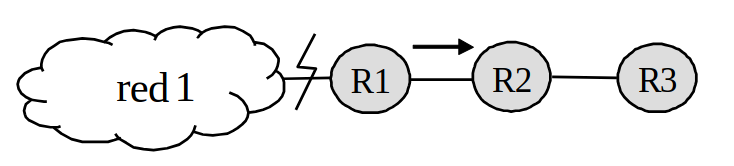
\includegraphics[width=0.6\linewidth]{./images/cuenta-infinito-rip.png}
    \label{fig:rip}
\end{figure}

Un problema que puede ocurrir es que algún camino se rompa y, dado la naturaleza del protocolo, esto tarda en notificarse. En el ejemplo que vemos arriba, R1 es notificado de que ya no es posible llegar a la red 1 por el camino que tenía aprendido. Pero R2, que aún no ha sido notificado, le comunica que él sabe llegar, por tanto R1 lo aprende. Cuando R2 se entera pasa un poco lo mismo, que aprende el camino por R1. Así pasa hasta el infinito (que en el caso de \acrshort{RIP} es equivalente a coste 16). Por esto a esto se le llama problema de la ``cuenta al infinito''. Veamos algunas posibles soluciones:
\begin{description}
    \item [Split horizon:] Se basa en que a un router se le prohíbe compartir una ruta por la misma interfaz por la que la aprendió en primer lugar.
    \item [Hold down:] Retrasa los mensajes que nos llegan de una dirección que ya conocemos 180 segundos, esperando a que nos respondan los anteriores, si siguen activos. 
    \item [Poison reverse:] Si no sabemos llegar a un destino, decimos que el coste es infinito (coste = 16).
\end{description}

\subsection{\acrfull{OSPF}}

Este protocolo permite definir el coste. Tiene un criterio por defecto, en el que el coste de un enlace es el inverso del ancho de banda (la velocidad) de dicho enlace. Busca el camino global que minimiza la suma de todos los costes usando Dijkstra. \\

Permite definir áreas, de forma que la difusión se hace en unas áreas concretas. Esto hace que sea mucho más escalable, al contrario que \acrshort{RIP}.\\

\noindent
Los mensajes que tenemos son:

\begin{itemize}
    \item Hello: para saludar a mis vecinos.
    \item Database description: para mandar la topología que conocemos. 
    \item Link status request/update/ack: para consultar o enviar cambios.
\end{itemize}


\subsection{Cabecera IP}
La cabecera IP tiene 20 Bytes. Veamos los campos, en orden, que la componen:
\begin{figure}[H]
    \centering
    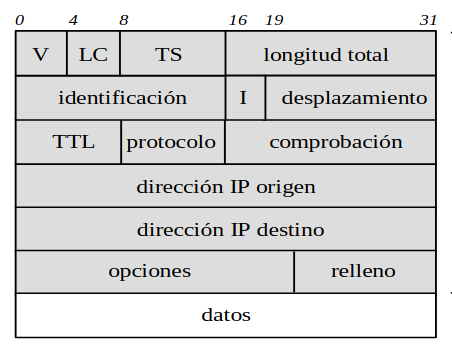
\includegraphics[width=0.4\linewidth]{./images/cabecera-ip.png}
\end{figure}

\begin{itemize}
    \item Versión (4 bits): La versión utilizada de \acrshort{IP}, 0100 si \acrshort{IPv4} y 0110 si \acrshort{IPv6}. 
    \item Tamaño de cabecera (4 bits): longitud de la cabecera IP en palabras de 32 bits. Como mínimo 5 palabras y como máximo 15 palabras.
    \item Tipo de Servicio (8 bits): hace referencia a la calidad de servicio deseada durante el tránsito del paquete por una red. Hay redes que ofrecer prioridades de servicios, considerando determinados tipos de paquetes más prioritarios que otros.
    \item Longitud total (16 bits): es el tamaño total, en octetos, del datagrama, incluyendo el tamaño de la cabecera y el de los datos.
    \item Identificador (16 bits): identificador único del datagrama. Se utiliza en caso de que el datagrama deba ser fragmentado, para poder distinguir los fragmentos de un datagrama de los de otro.
    \item Flags (3 bits): En la actualidad se utiliza para especificar valores relativos a la fragmentación.
        \begin{itemize}
            \item bit 0: Reservado, debe ser 0.
            \item bit 1 (DF): 0 = divisible; 1 = no divisible.
            \item bit 2 (MF): 0 = último fragmento; 1 = fragmento intermedio, le siguen más fragmentos. 
        \end{itemize}
    \item Desplazamiento (13 bits): en paquetes fragmentados indica la posición, en unidades de 64 bits, que ocupa dentro del datagrama original. 
    \item Tiempo de vida, \acrshort{TTL} (8 bits): indica el número de saltos máximo de un paquete en una red para evitar paquetes navegando en la red indefinidamente. En cada salto, el campo se reduce en una unidad, si llega a 0 se descarta.
    \item Protocolo (8 bits): tiene un identificador del protocolo de las capas superiores al que debe entregarse el paquete.
    \item Suma de Control de Cabecera (16 bits): es una comprobación de la corrección del datagrama. Se recalcula cada vez que algún nodo cambia alguno de sus campos. El método de cálculo consiste en suma en complemento a 1 cada palabra de 16 bits de la cabecera (poniendo 0 en este campo) y hacer el complemento a 1 del valor resultante. Así cuando llega al destino se hace esta misma operación y se comprueba si es correcta la cabecera.
    \item Dirección IP de origen (32 bits).
    \item Dirección IP de destino (32 bits).
    \item Opciones (opcional).
    \item Relleno: este campo tiene tantos como sea necesario para que la cabecera tenga un número de bits múltiplo de 32. 
\end{itemize}

\subsection{Fragmentación}
Las redes no permiten paquetes de cualquier tamaño. El tamaño máximo es $2^{16}$ Bytes, aunque ninguna red suele aceptar dicho tamaño. \\

Las redes cuentan con un \acrfull{MTU}: esta nos dice cuál es el tamaño máximo de lo que podemos transportar en la capa de datos a nivel de enlace, es decir, datos y cabecera de IP normalmente. \\ 

El \acrshort{MTU} depende del estándar de una tarjeta:
\begin{itemize}
    \item Ethernet: 1500 Bytes.
    \item Wifi: permite más pero normalmente el punto de acceso lo restringe a 1500 Bytes.
\end{itemize}

\noindent
Tenemos los siguientes campos en la cabecera de fragmentación:
\begin{itemize}
    \item Identificación: identifica al datagrama completo, no al paquete. Por esto, si un datagrama es fragmentado todos los fragmentos tendrán el mismo identificador.
    \item Campo de indicadores, como el \textit{more fragments}: si hay más fragmentos será un 1, y si es el último será un 0; o el \textit{don't fragment} que indica si un paquete puede ser fragmentado (si no puede y es necesario el paquete se descartará).
    \item Campo de desplazamiento (offset): sirve para ensamblar los paquetes en el destino. 
\end{itemize}

Algunas observaciones importantes:
\begin{itemize}
    \item Si hay algún error y no llegan todos los fragmentos de un datagrama se descarta todo y debe ser una capa superior la que se encargue de arreglar el problema.
    \item Solo fragmentamos cuando pasamos a un \acrshort{MTU} menor y solo se ensamblan en el destino, puesto que distintos fragmentos pueden seguir caminos distintos, dependiendo del encaminamiento.
\end{itemize}


\section{Asociación con la capa de enlace: el protocolo \acrshort{ARP}}
Cuando queremos enviar un paquete a un destino, mirando la tabla de encaminamiento sabemos la dirección IP del siguiente salto, pero para poder mandarle el paquete en el nivel de enlace necesitamos saber la dirección \acrshort{MAC}. \\

A diferencia de las direcciones IP origen y destino, que no cambian en ningún salto (salvo que se use \acrshort{NAT}); las direcciones MAC origen y destino cambian en cada reenvío del paquete, pues el nivel de enlace solo se encarga de encaminar punto a punto.\\

Entonces para mandar los paquetes necesitamos saber las direcciones MAC de los dispositivos. Esto se soluciona con el protocolo \acrfull{ARP}. 

\subsubsection{Funcionamiento}
Supongamos que A quiere mandar un paquete a B y tiene como intermediario a R1. A sabe la IP de R1 (por las tablas de encaminamiento) pero necesita saber la dirección MAC. 
\begin{itemize}
    \item A manda un ARP Request a nivel de enlace por la dirección FF:\ldots:FF (la dirección de difusión a nivel de enlace), preguntando por la MAC de la IP que conoce. 
    \item R1 contesta con un mensaje ARP Reply con su dirección MAC en unicast (es decir, respuesta única, no difusión) pues se conoce la MAC del que pregunta.
\end{itemize}

Este proceso no se hace siempre, sino se introduciría mucho tráfico. Las direcciones MAC que recibimos se van guardando en una caché y cuando pasa mucho tiempo expiran.\\

\begin{figure}[H]
    \centering
    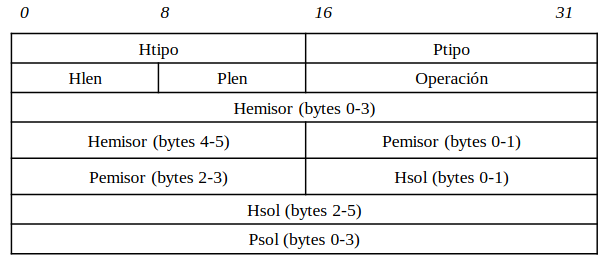
\includegraphics[width=0.6\linewidth]{./images/cabecera-arp.png}
\end{figure}


\noindent Campos de la cabecera: (H es referido a hardware, para nivel 2 para abajo; P es referido a protocolo, para nivel 3 para arriba):
\begin{itemize}
    \item Htipo: protocolo que se usa en el nivel de enlace.
    \item Ptipo: protocolo que se usa en el nivel de red.
    \item Hlen: longitud de la dirección hardware.
    \item Plen: longitud de la dirección del protocolo de red.
    \item Operación: Request o Reply.
    \item Hemisor: dirección hardware del emisor (MAC).
    \item Pemisor: dirección de red del emisor (IP).
    \item Hsol: dirección MAC del receptor.
    \item Psol: dirección IP del receptor.
\end{itemize}

Dependiendo de la operación que sea se rellenarán unos campos u otros.

\section{El protocolo \acrshort{ICMP}}
Es un protocolo que no es imprescindible pero ayuda. Sirve en general para informar al origen de que ha habido un error. Este protocolo es útil pues \acrshort{IP} no arregla ningún tipo de problema, pero al menos por este medio informa para que las capas superiores decidan si tomar acción.\\

Cuando ocurre un error, el equipo manda un paquete ICMP al origen. Es un nivel de red que se encapsula dentro de \acrshort{IP}. 

\subsubsection{Paquete \acrshort{ICMP}}
La cabecera es una palabra de 32 bits:
\begin{itemize}
    \item Tipo de mensaje, que indica el tipo de error que ocurrió.
    \item Código (subtipo de mensaje), para especificar más el error.
    \item Comprobación.
\end{itemize}

La parte de datos contiene los primeros 64 bytes del paquete que provocó el error, los 20 de la cabecera y 44 de datos del paquete IP. Esto es para ubicar el paquete que provocó el error.\\

De esta forma lo que tenemos es una cabecera IP y en la parte de datos un paquete ICMP, que a su vez se compone por una cabecera y en los datos tenemos una cabecera IP y algunos datos del paquete problemático.

\begin{figure}[H]
    \centering
    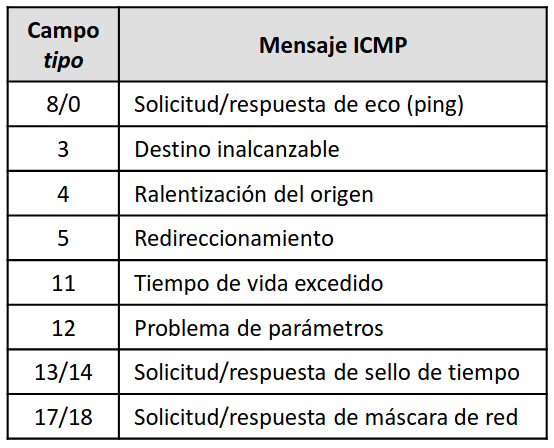
\includegraphics[width=0.4\linewidth]{./images/codigos-icmp.png}
    \label{fig:icmp}
\end{figure}

\section{Autoconfiguración de la capa de red (\acrfull{DHCP})}

Es un protocolo automático para asignar direcciones IP, máscaras, pasarelas por defecto e IP del servidor \acrshort{DNS}. Funciona a nivel de red pero se implementa en capa de aplicación, se encapsula en \acrshort{UDP}. \\

Al principio cuando no tenemos IP, la IP es 0.0.0.0. Para conseguir una IP se intercambian los siguientes mensajes entre el cliente y el servidor DHCP:
\begin{itemize}
    \item DHCP Discover: lo primero que hace es preguntar si hay alguien. 
    \item DHCP Offer: se presenta el servido y le ofrece una IP a usar. Esto es solo una oferta, no una imperativa.
    \item DHCP Request: el equipo comprueba si ya ha tenido una IP en la red y solicita tener esa IP en caso de que sí. 
    \item DHCP ACK: el servidor responde con la IP definitiva, y esta sí es imperativa. 
\end{itemize}

La IP destino usada en toda la transacción es la de difusión 255.255.255.255, y la de origen es la 0.0.0.0 en caso de ser el cliente o la del servidor DHCP en caso de ser el mismo. Los puertos usados son el 67 para el servidor y el 68 para el cliente.\\

Los pares pregunt-respuesta se etiquetan con un identificador de transacción para que el cliente sepa que el mensaje va para él.\\

\acrshort{DHCP} es un protocolo de \textit{leasing} o alquiler, la IP (y el resto de cosas) se asignan de forma temporal. Cuando tiempo va a expirar es necesario que el equipo mande una solicitud para que el servidor refresque el alquiler. El \textbf{DHCP release} se manda cuando queremos liberar la IP que se nos ha asignado, por ejemplo antes de que el dispositivo se apague. Sin embargo, si el servidor no recibe una petición del equipo antes de que se expire su alquiler libera la IP igualmente, dado que es posible que el equipo ya no la esté usando y sea necesario liberarla para no quedarnos sin IPs disponibles. 

\begin{observacion}
    Es posible configurar un servidor para que algunas IPs fijas se asignen a ciertos dispositivos.
\end{observacion}


